% ============================================================================
% Methodology. Fixed text, valid for every video. Times use \CuadrosPorSegundo (config.tex).
% Example figures: 180-frame test clip of DJI_0196 (700 x 700 px crop), times at f_r = 3 frames/s.
% ============================================================================
\section{Metodología de medición}\label{sec:metodo}

Para cada robot de la arena y en cada cuadro del video se mide la posición del centro, el vector
velocidad, la orientación acumulada $\theta$ y la velocidad angular $\omega$, con la cantidad de robots
$N$ fija. Las distancias se convierten a unidades SI con el diámetro real de los robots,
$D = \SI{\DiametroRobotCM}{\centi\metre}$, y los tiempos con la frecuencia de captura
$\fr$ (\cref{sec:escala}). Las figuras de ejemplo de esta sección provienen de un tramo de
\num{180}~cuadros de un ensayo con 22 robots (recorte de \num{700}\,$\times$\,\num{700}\,px),
expresado con $\fr = 3$~cuadros/s (\SI{60}{\second} reales).

\subsection{Flujo de procesamiento}

El análisis se divide en dos etapas (\cref{fig:flujo}). La etapa~A es la única que lee el video;
corregir un centro a mano, cambiar parámetros del seguimiento o recortar el tiempo solo vuelve a correr
la etapa~B, que tarda segundos.

\begin{figure}[H]
  \centering
  \begin{tikzpicture}[
      font=\small, node distance=4mm and 4mm,
      paso/.style={draw, rounded corners=3pt, align=center, minimum width=3.15cm, minimum height=1.25cm, fill=white},
      clave/.style={paso, draw=azul, very thick, fill=azul!10},
      ext/.style={paso, minimum height=0.95cm},
      flecha/.style={-stealth, thick, gray!70!black}]
    \node[paso]  (a1) {\textbf{Recorte}\\ tramo y ROI};
    \node[paso, right=of a1]  (a2) {\textbf{Calibración}\\ $r_{\mathrm{ext}}$, umbrales};
    \node[paso, right=of a2]  (a3) {\textbf{Detección}\\ anillo, trackpy};
    \node[clave, right=of a3] (a4) {\textbf{Candidatos}\\ posición, firma};
    \node[paso, below=14mm of a1] (b1) {\textbf{Seguimiento}\\ $N$ fijo};
    \node[paso, right=of b1]  (b2) {\textbf{Huecos}\\ interpolación};
    \node[paso, right=of b2]  (b3) {\textbf{Cinemática}\\ $\vec v$, $\theta$, $\omega$};
    \node[paso, right=of b3]  (b4) {\textbf{Vista del tramo}\\ sin re-analizar};
    \node[ext, below=8mm of b1] (c1) {Anclas manuales};
    \node[ext, below=8mm of b3] (c3) {Cambio de tramo};
    \node[ext, below=8mm of b4] (c4) {Exportaciones};
    \begin{scope}[on background layer]
      \node[draw=gray!60, fill=gray!8, rounded corners, inner sep=6pt, fit=(a1)(a4),
            label={[anchor=south west, font=\small\bfseries]north west:Etapa A: lee el video una vez}] {};
      \node[draw=gray!60, rounded corners, inner sep=6pt, fit=(b1)(b4),
            label={[anchor=south east, font=\small\bfseries]north east:Etapa B: sin leer el video}] {};
    \end{scope}
    \draw[flecha] (a1) -- (a2); \draw[flecha] (a2) -- (a3); \draw[flecha] (a3) -- (a4);
    \draw[flecha] (b1) -- (b2); \draw[flecha] (b2) -- (b3); \draw[flecha] (b3) -- (b4);
    \draw[flecha] (a4.south) -- ++(0,-5mm) -| (b1.north);
    \draw[flecha] (c1) -- (b1); \draw[flecha] (c3.north) -- ++(0,3mm) -| ($(b4.south west)!0.25!(b4.south east)$);
    \draw[flecha] ($(b4.south west)!0.75!(b4.south east)$) -- ($(c4.north west)!0.75!(c4.north east)$);
  \end{tikzpicture}
  \caption{Flujo de procesamiento.}
  \label{fig:flujo}
\end{figure}

\subsection{Sistema de referencia y unidades}

Las posiciones usan los ejes de la imagen: $x$ hacia la derecha, $y$ hacia abajo, con origen en la
esquina superior izquierda del recorte analizado. Los ángulos (dirección de la velocidad, $\theta$ y
$\omega$) son positivos en sentido antihorario visto en pantalla. La escala resulta de
\begin{equation}
  s = \frac{D}{2\,r_{\mathrm{ext}}}\quad\left[\si{\milli\metre\per px}\right],
\end{equation}
donde $r_{\mathrm{ext}}$ es el radio exterior del robot en píxeles medido por la calibración; su
incertidumbre (\SI{\pm 2}{\percent}) se propaga a todas las magnitudes en metros.

\paragraph{Video espejado.} Algunas cámaras graban la escena reflejada. Una reflexión invierte la
quiralidad: un giro horario se ve antihorario y viceversa. La opción \emph{Video espejado} de la
pestaña \emph{Seguimiento} corrige las exportaciones sin tocar el análisis, que siempre se hace sobre
la imagen tal como está (así la superposición coincide con el video). Para una reflexión respecto del
eje vertical de la imagen (\emph{horizontal}), con $W$ el ancho de la región analizada,
\begin{equation}
  x \to W - x,\qquad v_x \to -v_x,\qquad \theta \to -\theta,\qquad \omega \to -\omega ,
\end{equation}
y la dirección de la velocidad se recalcula; para una reflexión \emph{vertical} se cambian $y$ y $v_y$
en lugar de $x$ y $v_x$. El CSV lleva entonces la columna \texttt{espejo}, y las columnas
\texttt{x\_video\_px}, \texttt{y\_video\_px} quedan siempre en píxeles del archivo.

\begin{table}[H]
  \centering
  \caption{Magnitudes medidas.}
  \begin{tabular}{@{}llll@{}}
    \toprule
    Magnitud & Símbolo & Unidad & Definición \\
    \midrule
    Tiempo real & $t$ & \si{\second} & $t = n/\fr$, con $n$ el número de cuadro \\
    Posición & $x,\,y$ & \si{\metre} & centro del robot, ejes de imagen \\
    Velocidad & $v_x,\,v_y$ & \si{\metre\per\second} & $\mathrm{d}x/\mathrm{d}t$, $\mathrm{d}y/\mathrm{d}t$ \\
    Rapidez & $|\vec v|$ & \si{\metre\per\second} & $\sqrt{v_x^2+v_y^2}$ \\
    Dirección & $\varphi$ & \si{\degree} & $\operatorname{atan2}(-v_y,\,v_x)$; \SI{0}{\degree} = derecha \\
    Orientación & $\theta$ & \si{\degree} & giro acumulado desde el primer cuadro del tramo \\
    Velocidad angular & $\omega$ & \si{\degree\per\second}, \si{\radian\per\second} & $\mathrm{d}\theta/\mathrm{d}t$ \\
    \bottomrule
  \end{tabular}
\end{table}

\subsection{Calibración automática del tamaño}

Visto desde arriba, el robot es un disco claro (la pila) rodeado por un anillo oscuro (la placa).
Se usa una plantilla con un disco de radio $r_{\mathrm{int}} = 0{,}75\,r_{\mathrm{ext}}$ y un anillo
hasta $r_{\mathrm{ext}}$, y se barre $r_{\mathrm{ext}}$: la respuesta media de los $N$ picos más fuertes
es máxima cuando la plantilla coincide con el robot real (\cref{fig:calib}). A partir de
$r_{\mathrm{ext}}$ se derivan la escala de análisis ($24/r_{\mathrm{ext}}$, para trabajar siempre con
robots de unos \SI{24}{px} de radio), la separación mínima ($1{,}5\,r_{\mathrm{ext}}$) y el radio de
búsqueda del seguimiento ($0{,}625\,r_{\mathrm{ext}}$). Los umbrales de gris se fijan como fracción
del contraste medido entre anillo y disco, por lo que no dependen de la exposición.

\begin{figure}[H]
  \centering
  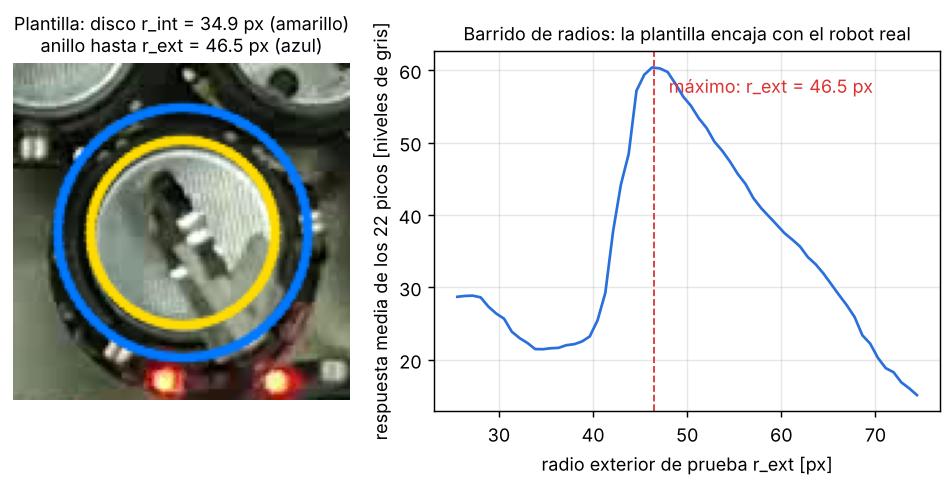
\includegraphics[width=0.9\linewidth]{figuras/metodo/f1_calibracion.png}
  \caption{Calibración: plantilla sobre un robot y respuesta en función del radio de prueba.}
  \label{fig:calib}
\end{figure}

\subsection{Detección}\label{sec:deteccion}

\paragraph{Filtro de anillo.} Para cada píxel se calculan el gris medio del disco y del anillo con
núcleos circulares normalizados, y se combinan como
\begin{equation}
  R(x,y) = \left(\mu_{\mathrm{disco}}-\mu_{\mathrm{anillo}}\right)\,
           \operatorname{clip}\!\left(\frac{G_{\max}-\mu_{\mathrm{anillo}}}{G_{\max}},\,0,\,1\right).
\end{equation}
El primer factor exige contraste; el segundo, que el anillo sea oscuro en valor absoluto. $R$ es alto
solo en los centros de los robots. En el código (\cref{lst:respuesta}), las medias locales son dos
convoluciones \texttt{cv2.filter2D} con núcleos normalizados a suma~1, calculadas sobre la imagen ya
reducida a la escala de análisis (los robots quedan con unos \SI{24}{px} de radio, lo que hace el
costo independiente de la resolución del video).

\begin{lstlisting}[caption={Filtro de anillo (\texttt{core/detection.py}).}, label=lst:respuesta]
def _disc_ring_kernels(r_in, r_out):
    R = int(np.ceil(r_out))
    yy, xx = np.mgrid[-R:R + 1, -R:R + 1]
    rr = np.hypot(xx, yy)
    disc = (rr <= r_in).astype(np.float32)
    ring = ((rr > r_in) & (rr <= r_out)).astype(np.float32)
    return disc / disc.sum(), ring / ring.sum()   # mean filters

def robot_response(gray, p):
    """Matched-filter map (uint8) at analysis scale."""
    ki, kr = _disc_ring_kernels(p.r_in * p.scale, p.r_out * p.scale)
    g = gray.astype(np.float32)
    m_disc = cv2.filter2D(g, -1, ki, borderType=cv2.BORDER_REFLECT)
    m_ring = cv2.filter2D(g, -1, kr, borderType=cv2.BORDER_REFLECT)
    gate = np.clip((p.ring_gray_max - m_ring) / p.ring_gray_max, 0.0, 1.0)
    return np.clip((m_disc - m_ring) * gate, 0, 255).astype(np.uint8)
\end{lstlisting}

\paragraph{Localización.} \texttt{trackpy.locate} busca los máximos locales de $R$ y devuelve su
centroide con precisión subpíxel. Se aplica sobre $R$ y no sobre la imagen porque la pila no es una
mancha uniforme: la palanca metálica y los reflejos corren el centroide. Los argumentos salen de la
calibración: el diámetro de la mancha buscada ($1{,}4\,r_{\mathrm{int}}$ en la escala de análisis,
redondeado a impar, porque el pico de $R$ es más angosto que el disco), la separación mínima entre
centros y \texttt{minmass}. Las coordenadas devueltas se dividen por la escala para volver a píxeles
del video (\cref{lst:locate}).

\begin{lstlisting}[caption={Llamada a trackpy (\texttt{core/detection.py}, función \texttt{locate}).}, label=lst:locate]
f = tp.locate(img, p.trackpy_diameter(), minmass=p.minmass,
              separation=max(1.0, p.separation * p.scale), invert=False)
f["x"] = f["x"] / p.scale          # back to video pixels
f["y"] = f["y"] / p.scale
\end{lstlisting}

\paragraph{Validación.} Un hueco de piso rodeado de robots también genera un pico, pero su ``anillo''
está formado por los vecinos y no es cerrado. Se trazan 360 rayos desde el centro y se exige que al
menos el \SI{82}{\percent} encuentre un píxel oscuro dentro de la banda del anillo
(\cref{fig:deteccion,fig:cobertura}). \texttt{cv2.warpPolar} desenrolla la imagen alrededor del
candidato: cada fila es un rayo y cada columna un radio, de modo que la cobertura es una sola
operación vectorizada (\cref{lst:cobertura}).

\begin{lstlisting}[caption={Cobertura angular del anillo oscuro (\texttt{core/detection.py}).}, label=lst:cobertura]
def ring_coverage(gray, x, y, r0, r1, dark):
    """Fraction of 360 rays whose darkest pixel in the band [r0, r1) is below `dark`."""
    r1i, r0i = int(np.ceil(r1)), int(max(0, np.floor(r0)))
    pol = cv2.warpPolar(gray, (r1i + 1, 360), (float(x), float(y)), r1i + 1,
                        cv2.WARP_POLAR_LINEAR)          # rows = angle, cols = radius
    return float((pol[:, r0i:r1i].min(axis=1) < dark).mean())
\end{lstlisting}

\begin{figure}[H]
  \centering
  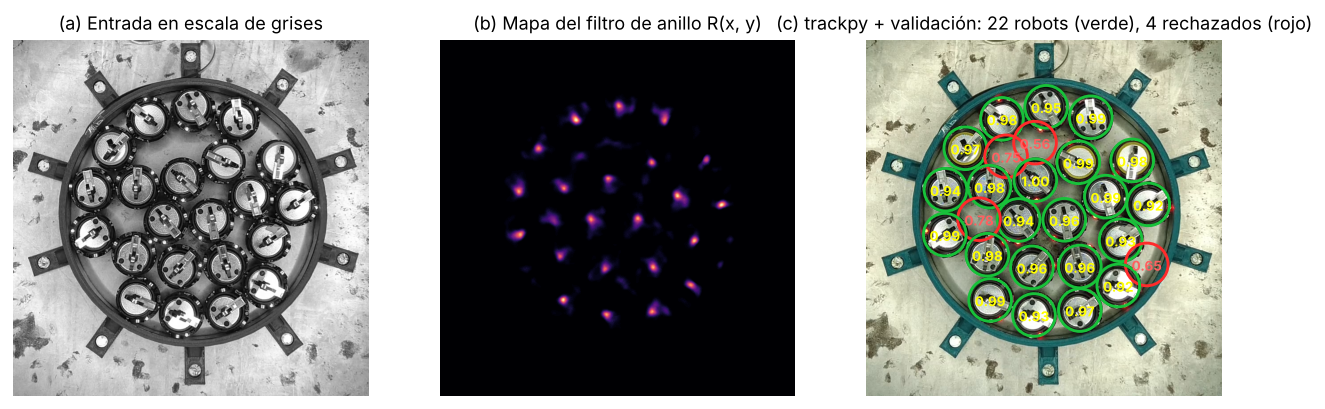
\includegraphics[width=\linewidth]{figuras/metodo/f2_deteccion.png}
  \caption{(a) Entrada. (b) Mapa $R$. (c) Candidatos con su cobertura: aceptados (verde) y huecos rechazados (rojo).}
  \label{fig:deteccion}
\end{figure}

\begin{figure}[H]
  \centering
  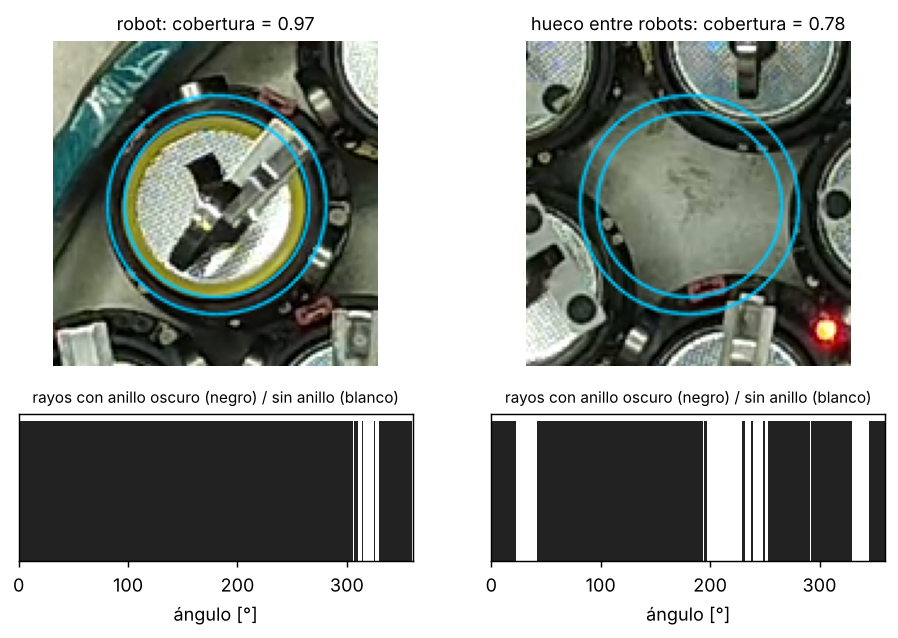
\includegraphics[width=0.72\linewidth]{figuras/metodo/f3_cobertura.png}
  \caption{Cobertura del anillo: un robot cierra el anillo en casi todos los rayos; un hueco, no.}
  \label{fig:cobertura}
\end{figure}

\subsection{Seguimiento con $N$ fijo}\label{sec:seguimiento}

En cada cuadro se predice la posición de cada robot (última posición más velocidad media reciente) y
se asignan predicciones y candidatos minimizando la distancia total (algoritmo húngaro), solo dentro
del radio de búsqueda. A los robots sin pareja se les ofrecen candidatos con umbrales relajados
(cobertura $\geq 0{,}70$ y luego $\geq 0{,}55$), pero solo cerca de su predicción. Un robot nuevo solo
se acepta si persiste en el \SI{75}{\percent} de los \Cuadros{20} siguientes. Los huecos acotados se
interpolan linealmente y cada punto queda con un estado (\cref{tab:estados}). Un centro marcado a mano
(ancla) es una restricción fija desde la que el seguimiento continúa (\cref{fig:seguimiento}).

El seguimiento corre en dos etapas. La etapa~A recorre el video una sola vez y guarda, para cada
cuadro, todos los candidatos con un umbral permisivo (cobertura $\geq 0{,}45$) y su firma de
rotación. La etapa~B trabaja solo sobre esa tabla: parte del cuadro con mejor detección y avanza
hacia adelante y hacia atrás. Cada robot guarda su última posición y una velocidad suavizada
exponencialmente ($\alpha = 0{,}5$); la predicción extrapola esa velocidad, limitada a
\texttt{max\_gap} cuadros para no alejarse demasiado en un hueco. La asignación usa
\texttt{scipy.optimize.linear\_sum\_assignment} con costo igual a la distancia, y costo prohibitivo
fuera del radio de búsqueda, que crece con la cantidad de cuadros sin detección
(\cref{lst:asignacion}).

\begin{lstlisting}[caption={Predicción y asignación con compuerta (\texttt{core/tracking.py}, resumido).}, label=lst:asignacion]
def predict(self, frame, max_gap):
    dt = frame - self.f                                   # signed: also runs backwards
    eff = np.sign(dt) * np.minimum(np.abs(dt), max_gap)   # damp long extrapolations
    return self.xy + self.v * eff[:, None], np.abs(dt)

def _gated_assign(pred, gates, cand):
    d = np.linalg.norm(pred[:, None, :] - cand[None, :, :], axis=2)
    cost = np.where(d <= gates[:, None], d, _BIG)          # outside the gate = forbidden
    r, c = linear_sum_assignment(cost)                    # Hungarian algorithm
    return [(i, j) for i, j in zip(r, c) if cost[i, j] < _BIG]

# per frame: manual anchors first, then the strict and the relaxed coverage levels
for cov_thr, gate_factor, status in levels:   # (0.82, 1, DETECTED), (0.70, 0.6, RELAXED), ...
    ks = np.flatnonzero(st.has & ~done)
    js = np.flatnonzero(~used & (cov >= cov_thr))
    for a, b in _gated_assign(pred[ks], base_gate[ks] * gate_factor, xy[js]):
        ...   # store position, status and candidate index; update the velocity
\end{lstlisting}

\begin{table}[H]
  \centering
  \caption{Estados de cada posición (columna \texttt{status}).}
  \label{tab:estados}
  \begin{tabular}{@{}lp{9.2cm}@{}}
    \toprule
    Estado & Significado \\
    \midrule
    detectado & asignado con el umbral estricto \\
    detectado (umbral relajado) & asignado con cobertura 0,55--0,82 cerca de la predicción \\
    manual & centro marcado a mano \\
    interpolado & hueco de hasta \Cuadros{15} entre dos detecciones (advertencia) \\
    predicho (revisar) & hueco más largo o sin detección de un lado (error) \\
    perdido & sin ninguna posición \\
    \bottomrule
  \end{tabular}
\end{table}

\begin{figure}[H]
  \centering
  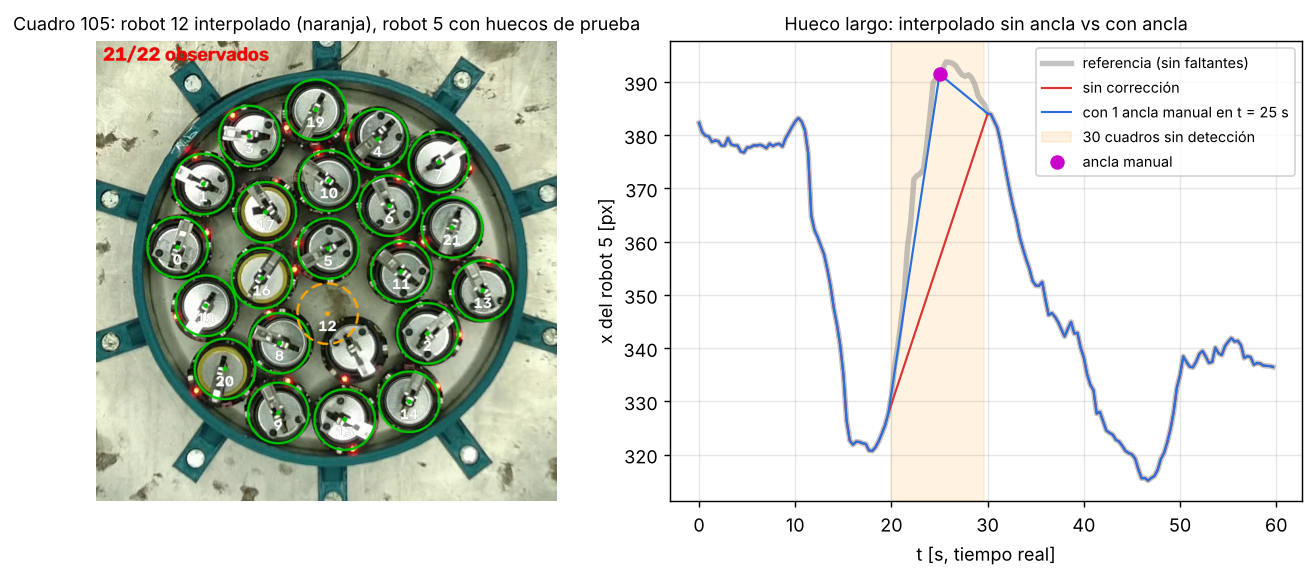
\includegraphics[width=\linewidth]{figuras/metodo/f4_seguimiento.png}
  \caption{Faltantes simulados: robot interpolado (naranja) y efecto de una sola ancla manual en un
    hueco de \Cuadros{30}. Tiempo real con $\fr = 3$~cuadros/s.}
  \label{fig:seguimiento}
\end{figure}

\subsection{Velocidad}\label{sec:velocidad}

El centro detectado fluctúa entre 1 y \SI{5}{px} por cuadro; una diferencia finita multiplicaría ese
ruido por $\fr$. Por eso la velocidad se obtiene con un filtro de Savitzky--Golay: para cada instante
se ajusta por mínimos cuadrados un polinomio de grado~2 a los cuadros vecinos (ventana de
\Cuadros{7} por defecto) y se toma su derivada analítica,
\begin{equation}
  v_x(t_i)=\left.\frac{\mathrm{d}\hat p_i}{\mathrm{d}t}\right|_{t_i},\qquad
  \hat p_i=\arg\min_{p\in\mathbb P_2}\sum_{j=-3}^{3}\bigl[x(t_{i+j})-p(t_{i+j})\bigr]^2 ,
\end{equation}
con $t_{i+j} = (i+j)/\fr$, y lo mismo para $v_y$ (\cref{fig:velocidad}). Una ventana mayor reduce
el ruido pero atenúa los cambios bruscos, como los choques. La ventana $w$ es un número de cuadros
(campo \emph{Suavizado} de la pestaña \emph{Seguimiento}): su duración real es $w/\fr$ y crece si
la captura es más lenta. En el código, \texttt{scipy.signal.savgol\_filter} con \texttt{deriv=1} y
\texttt{delta}$\,=1/\fr$ devuelve directamente la derivada por segundo real; los huecos
(\texttt{NaN}) se rellenan por interpolación solo para filtrar y se vuelven a marcar después
(\cref{lst:derivada}). La escala espacial se aplica al final:
$v\,[\si{\metre\per\second}] = v\,[\si{px\per\second}]\cdot s$.

\begin{lstlisting}[caption={Derivada temporal suavizada (\texttt{core/kinematics.py}).}, label=lst:derivada]
def _derivative(v, fps, p):
    """d/dt along axis 0 for each column; NaNs are bridged by interpolation, then restored."""
    out = np.full_like(v, np.nan, dtype=float)
    n = len(v)
    for k in range(v.shape[1]):                       # one column per robot
        col = v[:, k]
        ok = np.isfinite(col)
        if ok.sum() < 2:
            continue
        idx = np.arange(n)
        filled = np.interp(idx, idx[ok], col[ok])
        w = _odd_window(p.window, n, p.polyorder)
        d = savgol_filter(filled, w, p.polyorder, deriv=1, delta=1.0 / fps, mode="interp")
        d[~ok] = np.nan
        out[:, k] = d
    return out
\end{lstlisting}

\begin{figure}[H]
  \centering
  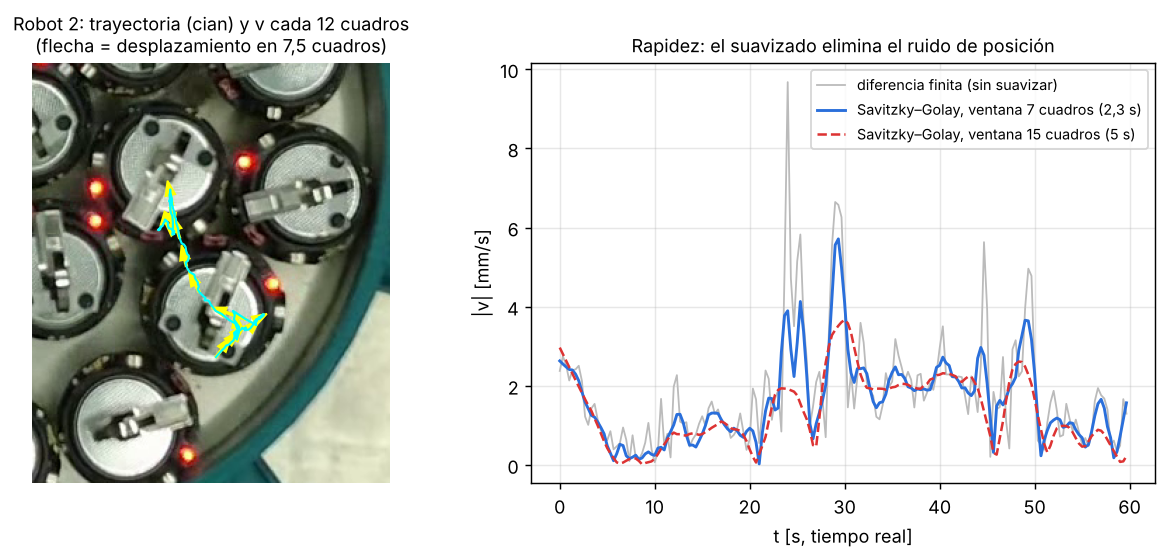
\includegraphics[width=\linewidth]{figuras/metodo/f5_velocidad.png}
  \caption{Trayectoria y vector velocidad de un robot (la flecha mide el desplazamiento en
    \num{7.5}~cuadros, por lo que su largo no depende de $\fr$); rapidez en tiempo real sin suavizar
    y con Savitzky--Golay, con $\fr = 3$~cuadros/s.}
  \label{fig:velocidad}
\end{figure}

\subsection{Orientación y velocidad angular}\label{sec:rotacion}

\paragraph{Firma de rotación.} Alrededor de cada centro la imagen se desenrolla en coordenadas
polares; una rotación del robot es entonces un corrimiento a lo largo del eje angular. En dos bandas
(pila, $0{,}15$--$0{,}70\,r_{\mathrm{ext}}$, y anillo, $0{,}75$--$0{,}95\,r_{\mathrm{ext}}$) se guarda el
perfil angular normalizado como sus primeros $K=12$ armónicos de Fourier (\cref{lst:firma}). Restar
la media de cada radio antes de promediar la banda elimina el gradiente radial de iluminación, y
normalizar por el desvío hace a la firma insensible al brillo de la escena.

\begin{lstlisting}[caption={Firma de rotación de un robot (\texttt{core/rotation.py}, resumido).}, label=lst:firma]
pol = cv2.warpPolar(gray, (R, 128), (x, y), R, cv2.WARP_POLAR_LINEAR)  # 128 angles x R radii
for b, (r0, r1) in enumerate(((0.15, 0.70), (0.75, 0.95))):            # battery, PCB ring
    band = pol[:, int(r0 * R):int(r1 * R)]
    prof = (band - band.mean(axis=0, keepdims=True)).mean(axis=1)      # angular profile
    prof = (prof - prof.mean()) / prof.std()
    sig[b] = np.fft.fft(prof)[1:13] / 128                              # harmonics 1..12
\end{lstlisting}

\paragraph{Ángulo entre dos cuadros.} El giro relativo es el máximo de la correlación circular de las
firmas,
\begin{equation}
  c(\Delta)=\operatorname{Re}\sum_b\sum_{k=1}^{K} S_2[b,k]\,\overline{S_1[b,k]}\,e^{ik\Delta},\qquad
  \Delta\theta=\arg\max_\Delta c(\Delta),
\end{equation}
refinado con dos pasos de Newton (error mediano \SI{0.37}{\degree} con rotaciones conocidas). Como
$c(\Delta)$ solo tiene armónicos hasta $K$, una grilla de 128 puntos (por FFT inversa) ubica el
máximo y la derivada analítica lo refina (\cref{lst:angulo}).

\begin{lstlisting}[caption={Giro relativo entre dos firmas (\texttt{core/rotation.py}, resumido).}, label=lst:angulo]
C = (s2 * np.conj(s1)).sum(axis=-2)                 # cross-spectrum, summed over bands
spec[..., 1:K + 1] = C
c = np.real(np.fft.ifft(spec, axis=-1)) * 128        # c(Delta) on a 128-point grid
d = np.argmax(c, axis=-1) * (2 * np.pi / 128)
k = np.arange(1, K + 1)
for _ in range(2):                                   # Newton on dc/dDelta = 0
    e = C * np.exp(1j * k * d[..., None])
    d1 = np.real((1j * k * e).sum(-1))
    d2 = np.real((-(k ** 2) * e).sum(-1))
    d = d - np.where(d2 < 0, d1 / d2, 0.0)
angle = -((np.degrees(d) + 180) % 360 - 180)         # CCW on screen (warpPolar is clockwise)
\end{lstlisting}

\paragraph{Ángulo acumulado.} Sumar solo giros entre cuadros consecutivos acumula el error de cada
paso. Cada cuadro se compara con los que están 1, 2, 4, 8 y 16 cuadros atrás y todos los ángulos se
resuelven juntos por mínimos cuadrados ponderados por la similitud $q$:
\begin{equation}
  \min_{\theta}\sum_{(i,L)} q_{i,L}\left(\theta_{i+L}-\theta_i-m_{i,L}\right)^2,\qquad \theta_0=0,
\end{equation}
con un error acumulado $\leq \SI{2}{\degree}$ en \num{3000}~cuadros. El sistema es ralo y de banda
(cada ecuación vincula dos cuadros separados a lo sumo 16), por lo que se arma con
\texttt{scipy.sparse.coo\_matrix} y se resuelve con las ecuaciones normales y \texttt{spsolve}, en
tiempo proporcional a la cantidad de cuadros. Las comparaciones largas con similitud $q<0{,}8$ o
que discrepan más de \SI{30}{\degree} de la cadena incremental se descartan. Finalmente
$\omega=\mathrm{d}\theta/\mathrm{d}t = \fr\,\mathrm{d}\theta/\mathrm{d}n$ con el mismo
Savitzky--Golay (\cref{fig:rotacion}). La
\cref{fig:desrotacion} verifica la medición: al girar cada imagen por $-\theta$, los LEDs y los puntos
de la placa quedan fijos, por lo que $\theta$ describe la orientación del cuerpo del robot (la palanca
de la pila gira levemente respecto de él y no sirve como referencia).

\begin{figure}[H]
  \centering
  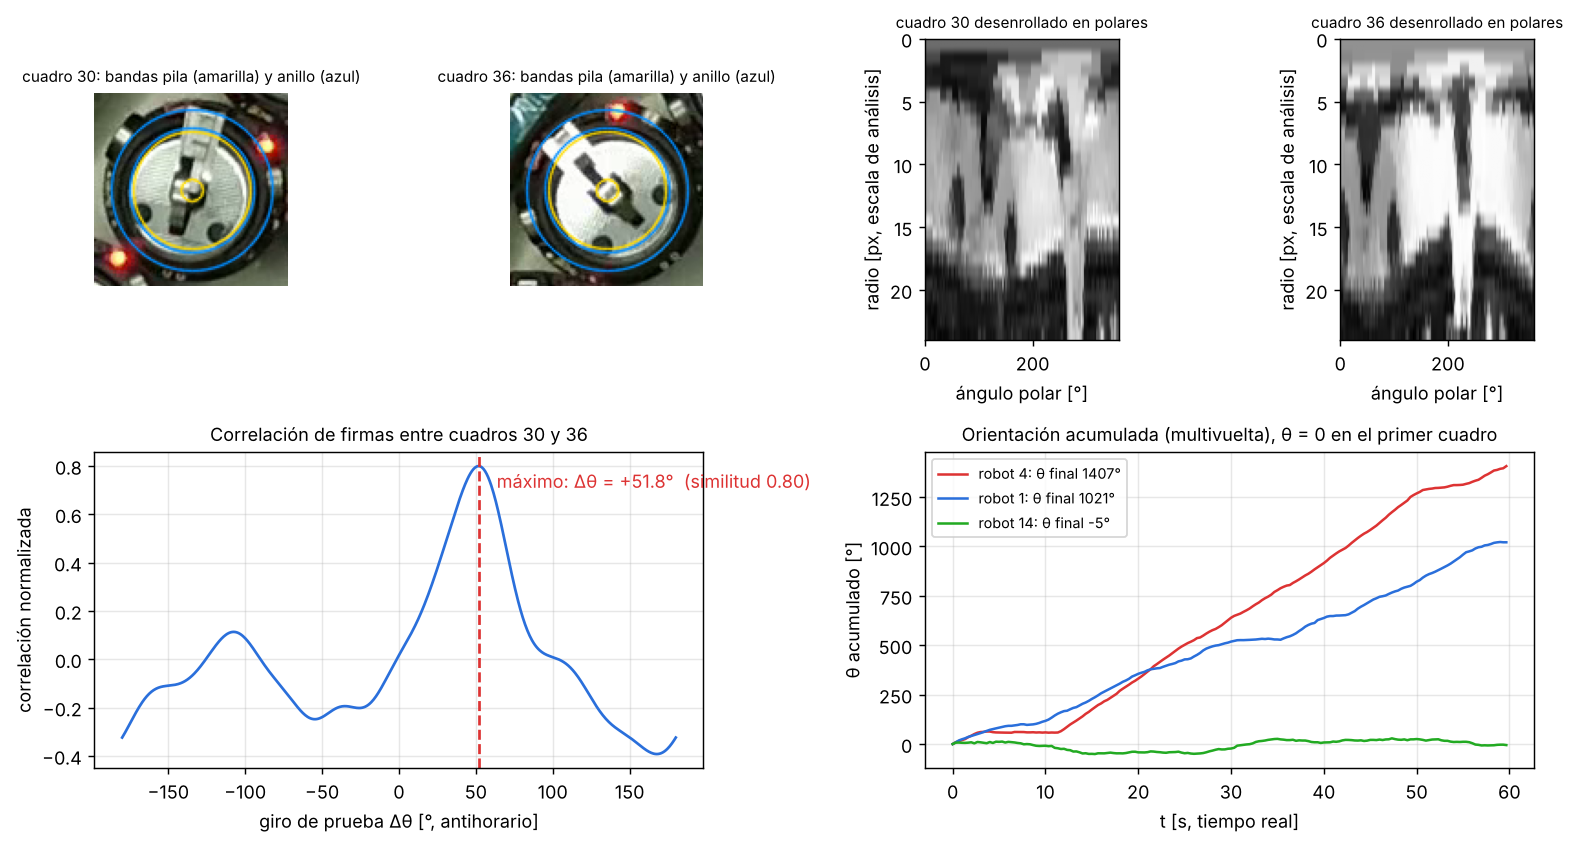
\includegraphics[width=\linewidth]{figuras/metodo/f6_rotacion.png}
  \caption{Firma polar en dos cuadros, correlación de las firmas y orientación acumulada de tres robots.}
  \label{fig:rotacion}
\end{figure}

\begin{figure}[H]
  \centering
  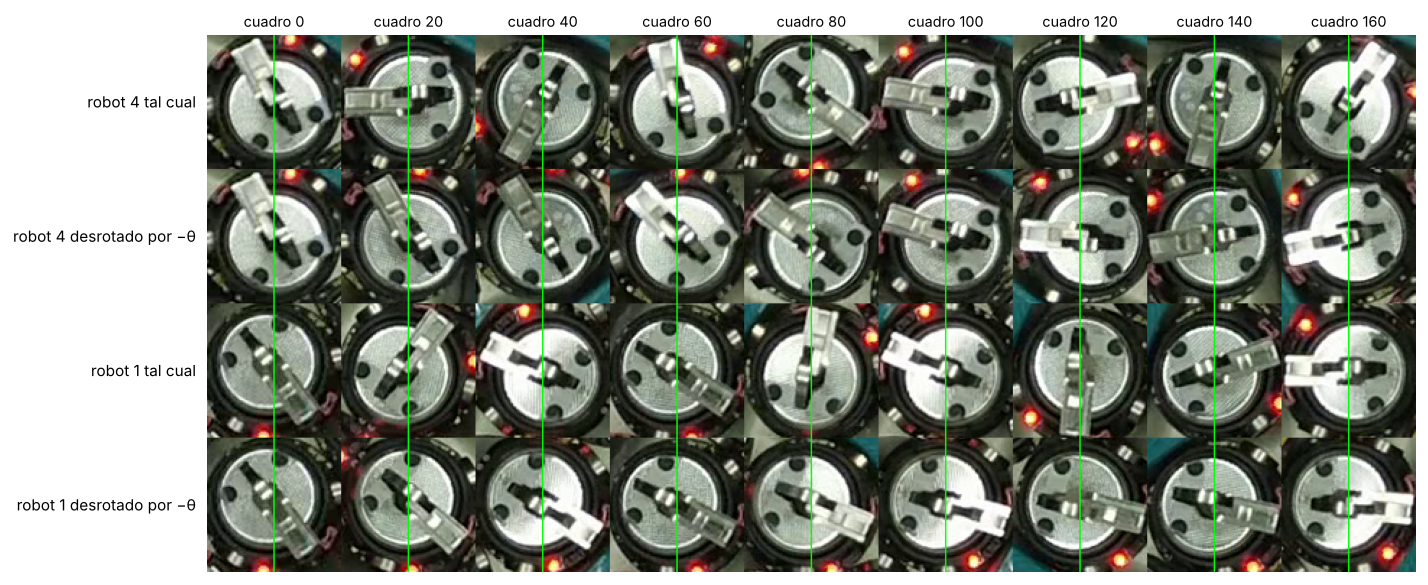
\includegraphics[width=\linewidth]{figuras/metodo/f7_desrotacion.png}
  \caption{Validación por desrotación: filas pares, las imágenes de la fila anterior giradas por $-\theta$.}
  \label{fig:desrotacion}
\end{figure}

\begin{figure}[H]
  \centering
  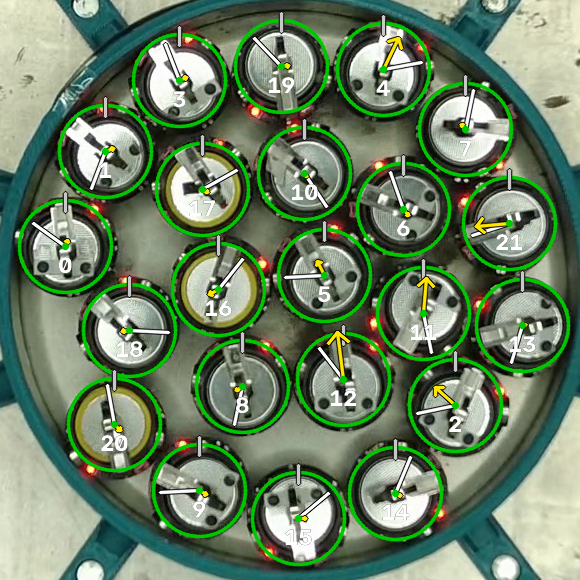
\includegraphics[width=0.6\linewidth]{figuras/metodo/f8_superposicion.png}
  \caption{Superposición en la aplicación: estado (color del círculo), velocidad (flecha amarilla,
    desplazamiento en \num{7.5}~cuadros) y orientación (aguja blanca; la marca a las 12~h es $\theta=0$).}
  \label{fig:superposicion}
\end{figure}

\subsection{Recorte temporal}

Si se recorta el tiempo después de analizar, los resultados se toman del análisis completo: las
derivadas conservan su precisión en los bordes y $\theta$ se re-referencia a cero en el primer cuadro
del tramo. Las exportaciones y este informe usan siempre el tramo vigente (\cref{sec:procedimiento}).

\subsection{Incertidumbres y limitaciones}

\begin{itemize}
  \item Posición: fluctuación de 1--\SI{5}{px} entre cuadros; escala espacial: \SI{\pm 2}{\percent}.
  \item Escala temporal: un error relativo en $\fr$ pasa sin atenuar a $|\vec v|$ y a $\omega$,
        según la \cref{eq:incert_t}; con $\fr$ estimado de la configuración de la cámara o del registro del
        sensor es del orden de \SI{1}{\percent}, con la duración nominal del nombre puede superar el
        \SI{10}{\percent}.
  \item Velocidad: los cambios más cortos que la ventana de suavizado (\EnSeg{7}) se atenúan, y nada
        más rápido que $\Delta t = \EnSeg{1}$ se resuelve.
  \item Orientación: \SI{\pm 0.4}{\degree} por comparación, $\leq \SI{2}{\degree}$ acumulado; en cuadros
        sin imagen del robot $\theta$ se interpola, y un giro mayor que media vuelta entre dos
        cuadros comparados no se detecta.
  \item Huecos: la interpolación lineal se aparta si el robot cambia de dirección; tras un hueco, un
        candidato aceptado con umbral relajado puede ser un falso positivo cercano a una predicción
        errónea. Para estadística conviene usar solo \texttt{status} = detectado.
\end{itemize}
